\section*{Results and discussion}

\subsection*{SGL accurately predicts age from tractometry data in a regression setting}

To test the performance of SGL in tractometry data in a continuous regression
task, we focus here on the prediction of biological age from the tractometry
data. Prediction of ``brain age'' is a commonly undertaken task. This is both
because it operates on a natural scale, with meaningful and easily understood
units, as well as because predictions of brain age, and deviations from accurate
prediction are diagnostic of overall brain health (for a recent review, see
\cite{Cole2019-rz}). The WH dataset used here contains data from 76 healthy
subjects, ranging between 6 years and 50 years of age
\cite{yeatman2014lifespan}. In this case, biological age was used as the
predicted variable ($y$ in equation \ref{eq:lm}). SGL was fit to
tractometry-extracted features: FA and MD in 20 major brain tracts, with each
tract divided into 100 nodes. To evaluate the fit of the model, we used a nested
cross-validation procedure. In this procedure, batches of subjects are held out.
For each batch (or fold), the model is fully fit without this data. Then, once
the parameters are fixed, the model is inverted to predict the ages of held out
subjects based on the linear coeffiecients and the static non-linearity. data is
held out, and a model age was predicted using a model that was fit without that
subject. This scheme automatically finds the right level of regularization and
fits the coefficients to the ill-posed linear model, while guarding against
overfitting. SGL accurately predicts the age of the subjects in this procedure,
with a mean absolute error of 3.6 years (Figure \ref{fig:regress-results}, left
panel). This is lower than the results of a recent study that predicted age in a
large sample, based on diffusion MRI features \cite{Richard2018-ux}.
Nevertheless, older subjects have higher residual variance, reflecting the
automatically-chosen log-transformation and implying that brain age becomes more
difficult to predict as we age chronologically (\ref{fig:regress-results}, right
panel). The model weights are distributed over many different tracts and dMRI
tissue properties (Figure \ref{fig:regress-beta} left). This demonstrates that
SGL is not coerced to produce overly sparse results when a more accurate model
requires a dense selection of features. Furthermore, looking closer at a
selection of tracts where high coefficients are found demonstrates that
diffusion properties (FA, in this case) are different in different age groups in
parts of the tracts where these higher coefficients are found (Figure
\ref{fig:regress-beta} right).


\begin{figure}[!h]
    \centering
    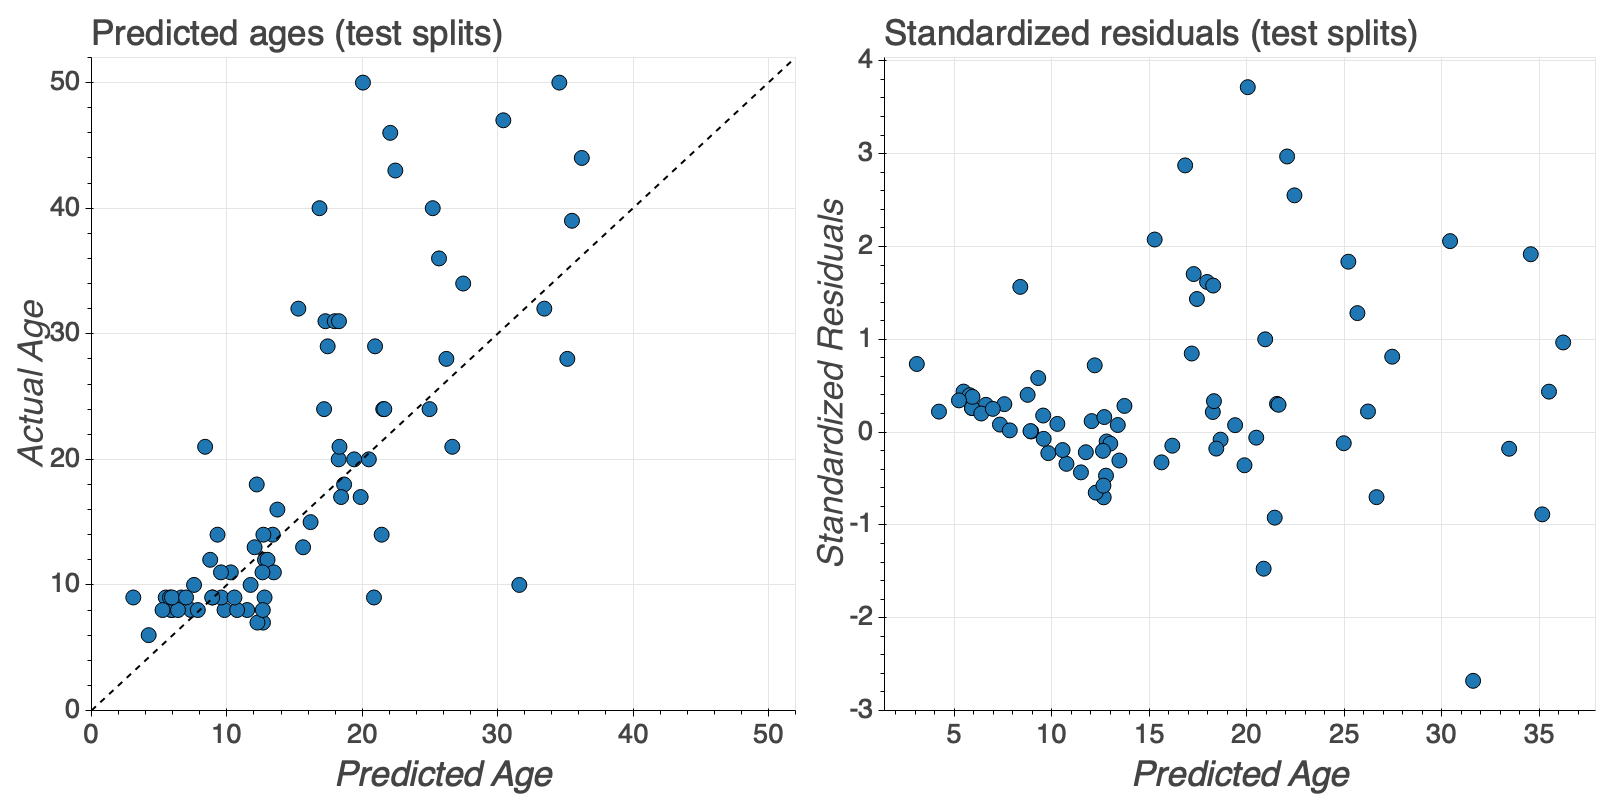
\includegraphics[width=0.8\textwidth]{regression_residuals.png}
    \caption{{\bf Predicting age with tractometry and SGL.} Left: The predicted
    age of each individual (on the abscissa) and true age (on the ordinate),
    from the test splits (i.e., when each subject's data was held out in fitting
    the model); an accurate prediction falls close to the $y=x$ line (dashed).
    The mean absolute error in this case is 3.6 years and, the coefficient of
    determination $R^2=0.3$. Right: Standardized residuals (on the abscissa) as
    a function of the true age (on the ordinate). Predictions are generally more
    accurate for younger individuals.}
    \label{fig:regress-results}
\end{figure}

\begin{figure}[!h]
    \centering
    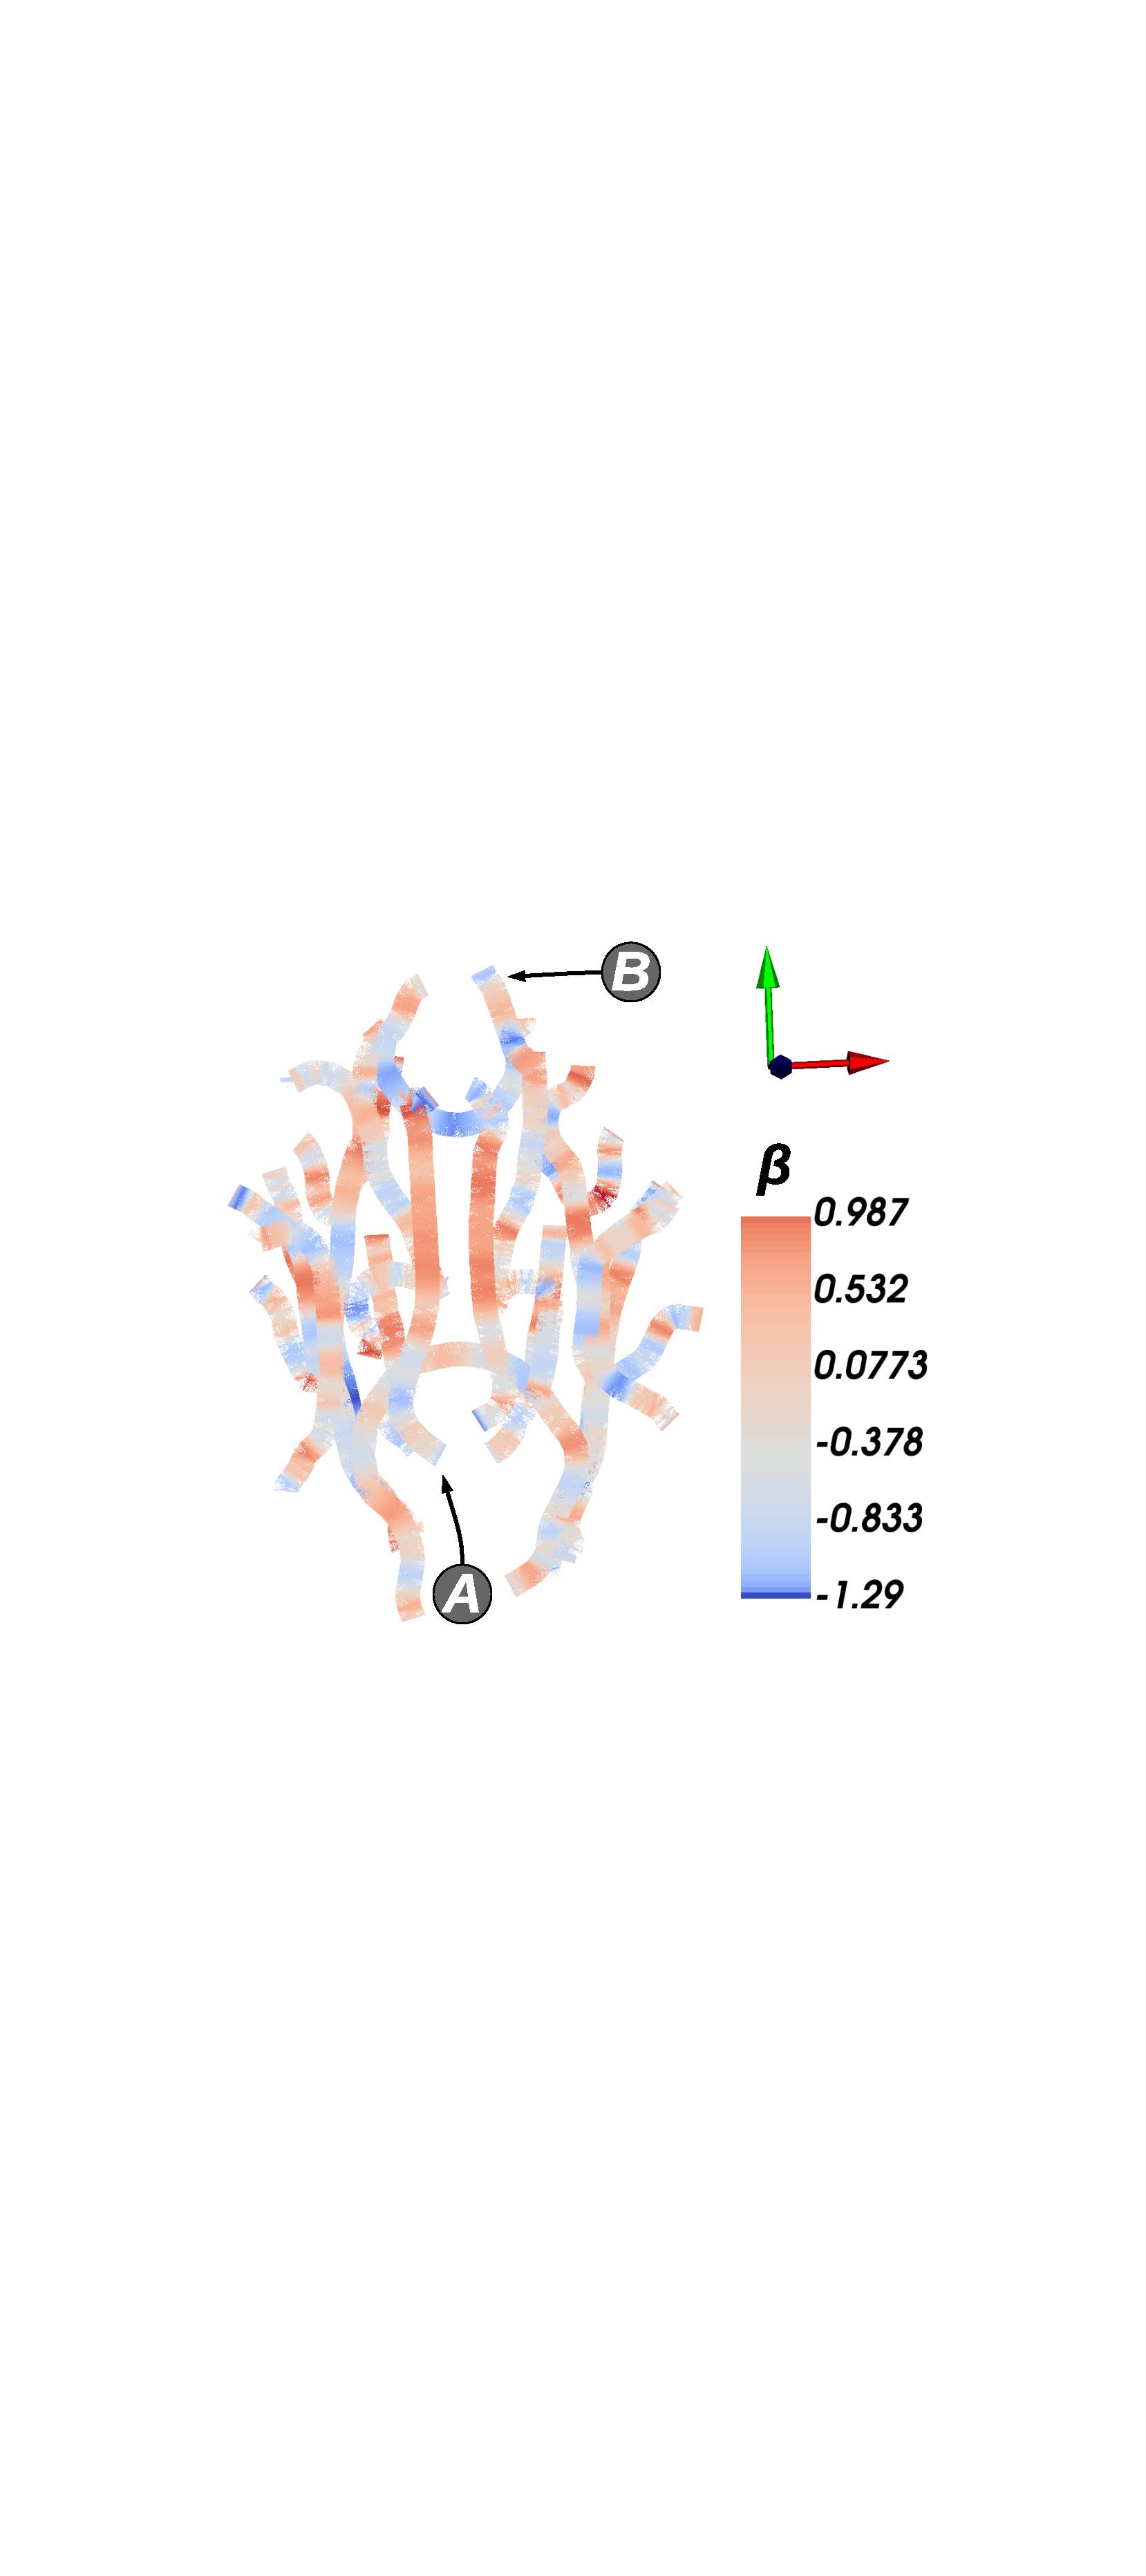
\includegraphics[width=0.3\textwidth]{regression_beta_annotated.pdf}
    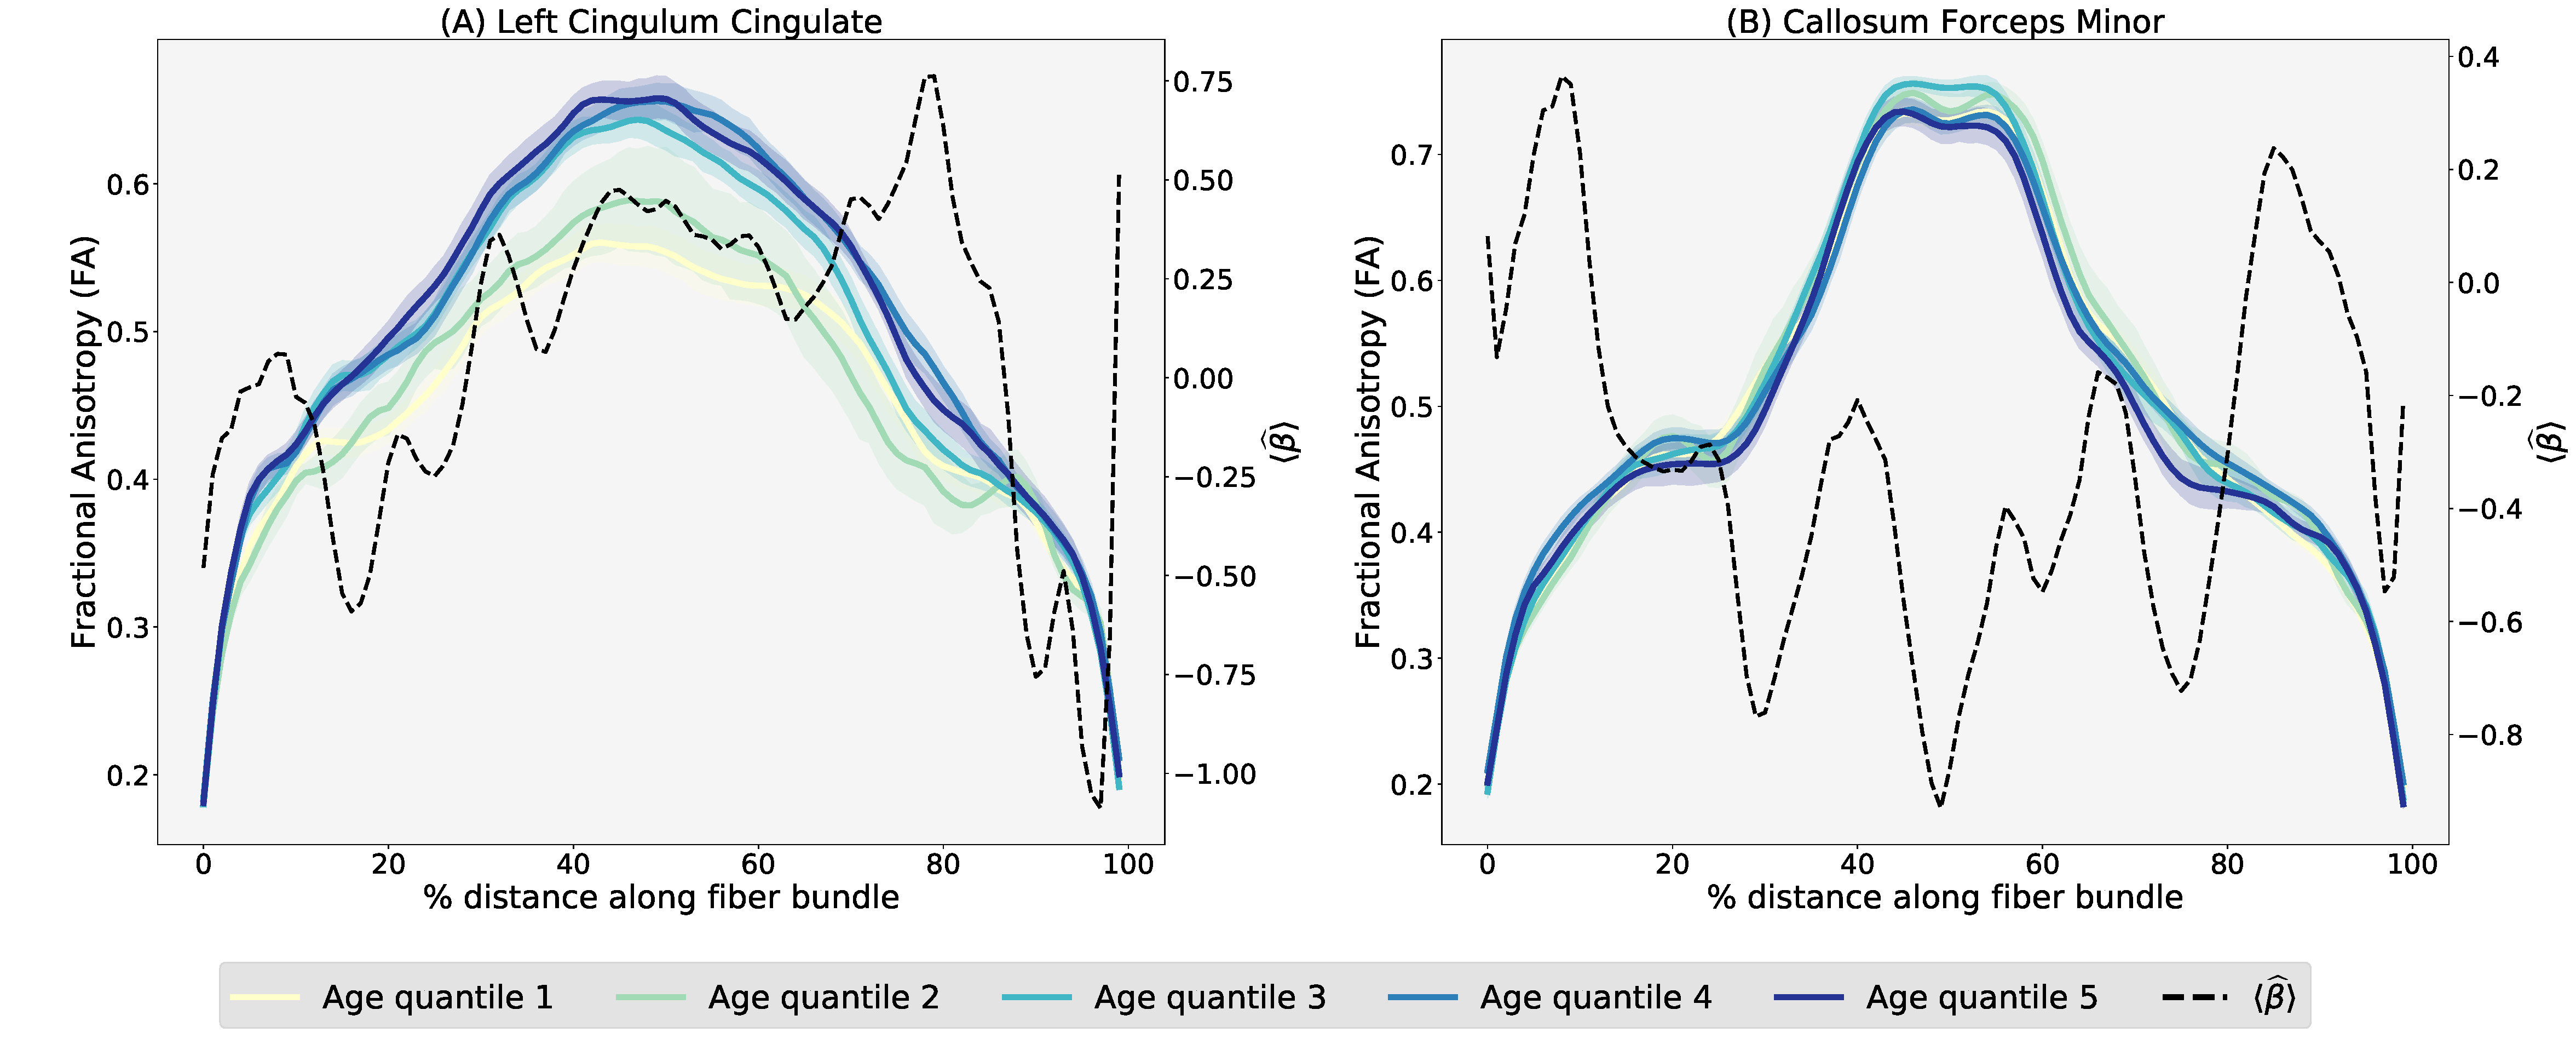
\includegraphics[width=0.67\textwidth]{regression_tract_profiles.pdf}
    \caption{{\bf Feature importance for predicting age from tractometry.} Left:
    A skeletonized display of the main brain tracts analyzed, with anterior
    facing up, and right hemisphere on the right. The $\hat{\beta}$ coefficients
    displayed in blue (negative) to red (positive) are for measurements of FA
    along the length of the tracts. The left cingulum cingulate (A) and forceps
    minor (B) are highlighted. Right: the FA (in shades of blue and green) and
    the $beta$ coefficients (dashed) in (A) left cingulum and (B) forceps
    minor.}
    \label{fig:regress-beta}
\end{figure}

\subsection*{SGL accurately detects ALS in tractometry data in a classification setting}

Using data from a previous study of the corticospinal tract (CST) profile and
ALS\cite{sarica2017corticospinal}, we tested the performance of SGL in a
classification setting. The previous study predicted ALS status with a mean
accuracy of 80\% using a random forest algorithm based on a priori selection of
features within the corticospinal tract. SGL delivers competitive predictive
performance (mean 93\% $\pm$ 2\% accuracy, 0.978 $\pm$ 0.006 ROC AUC) without
the need for a priori feature engineering. The results of the classification
prediction are shown in Fig~\ref{fig:class-results}, with ``ground-truth'' ALS
status separated into columns, and predicted ALS status encoded by color. In
addition to this classification performance, SGL also identifies the white
matter tracts most important for ALS classification. The relative importance of
white matter features is captured in the $\beta$ coefficients from
Eq~\eqref{eq:sgl}. Fig~\ref{fig:class-beta} depicts these coefficients across
the brain, laid out on a skeleton of the major tracts. We find that SGL selects
FA metrics in the corticospinal tract and particualrly in the right
corticospinal tract as most important to ALS classification, confirming previous
findings\cite{van2011upper, toosy2003diffusion, sarica2014tractography,
sage2007quantitative, sage2009quantitative, karlsborg2004corticospinal,
ellis1999diffusion, cosottini2005diffusion, ciccarelli2009investigation,
abe2010voxel} and identifying exactly the portions of the brain that were
selected \emph{a priori} in the previous study from which we collected our
data\cite{sarica2017corticospinal}.

\begin{figure}[!h]
    \centering
    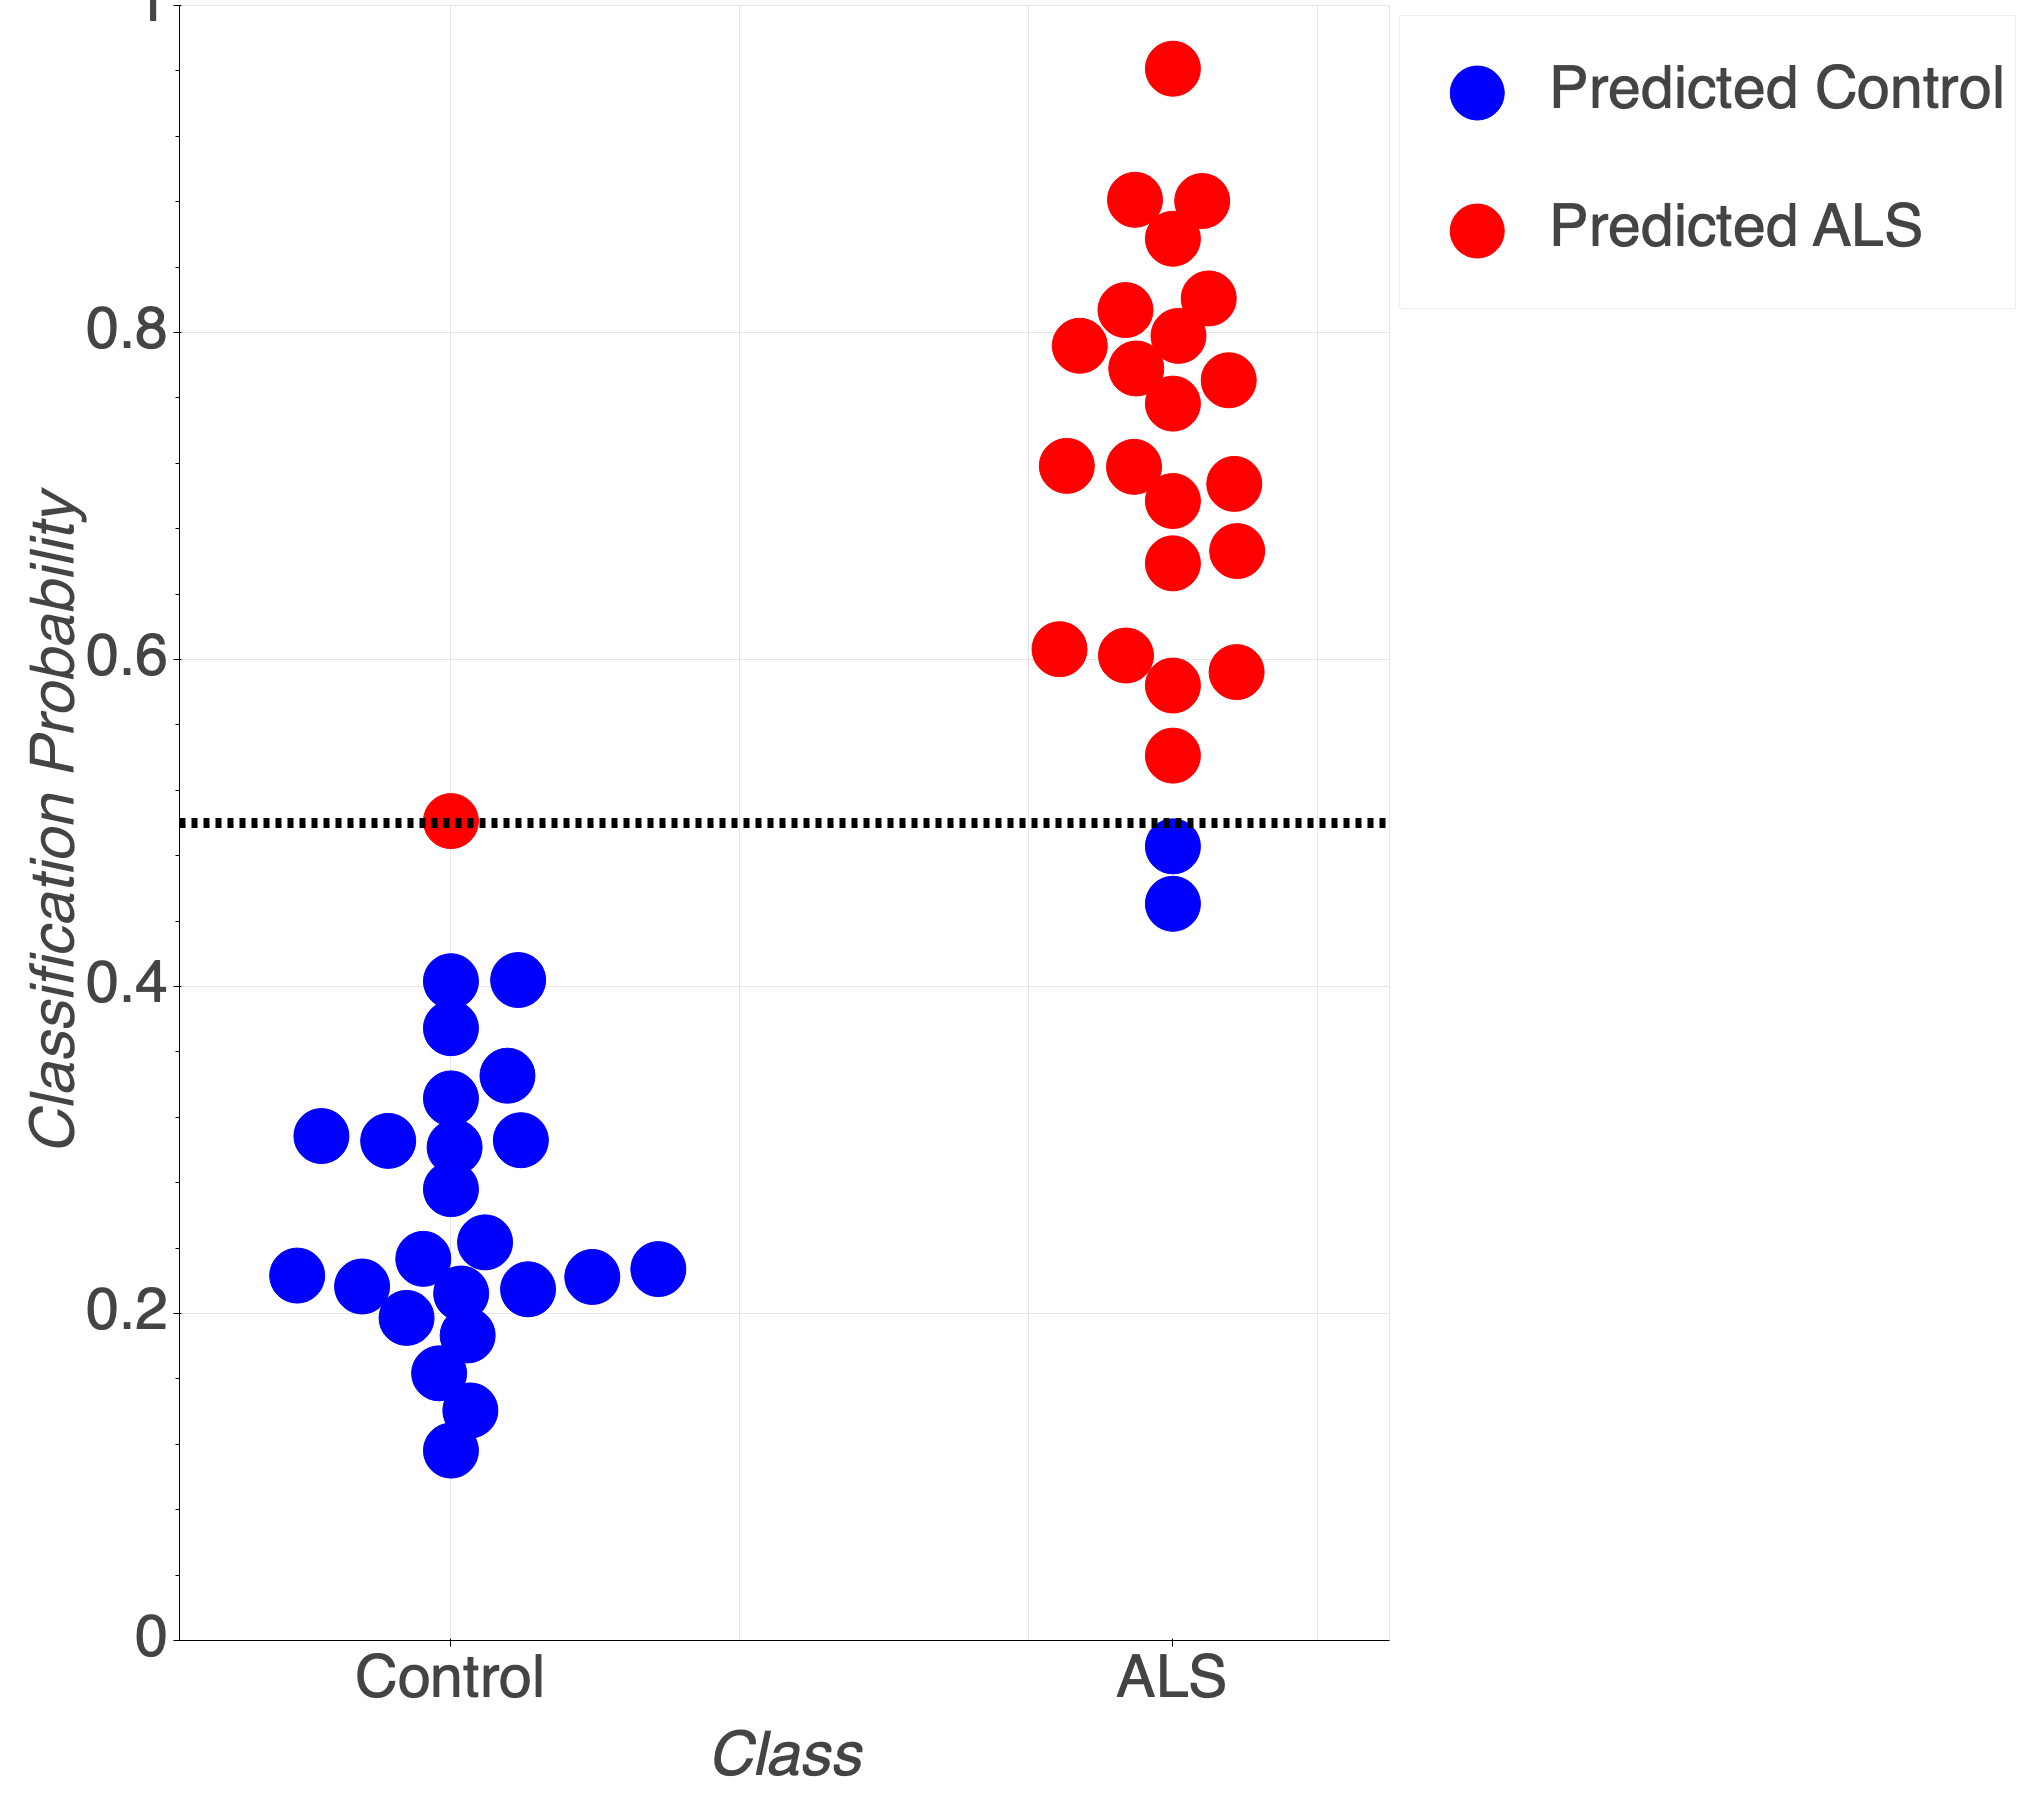
\includegraphics[width=0.45\textwidth]{classification_probs.png}
    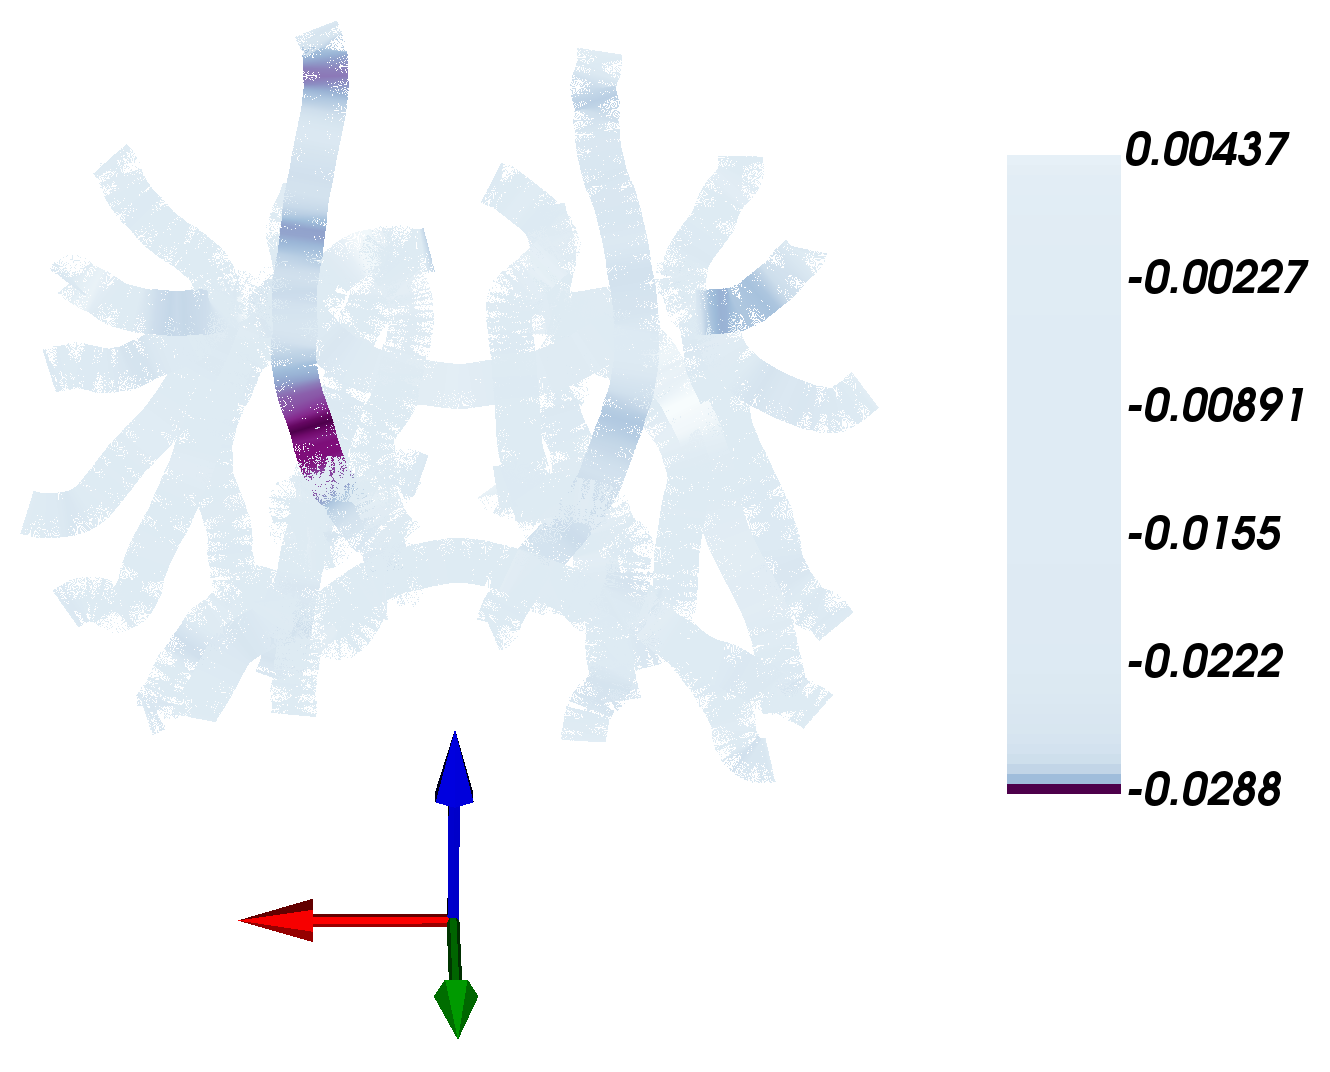
\includegraphics[width=0.45\textwidth]{classification_beta_bupu.png}

    \caption{{\bf SGL accurately predicts ALS.}
        Left: Classification probabilities for each subject's ALS diagnosis.
        Controls are on the left while patients are on the right. Predicted
        controls are in blue and predicted patients are in red. Thus, false
        positive are represented as red dots on the left, while false negatives
        are represented as blue dots on the right. The SGL algorithm achieves
        93\% $\pm$ 2\% accuracy,with 0.978 $\pm$ 0.006 ROC AUC. Right: SGL
        coefficients are presented on a skeleton of the major tracts. The brain
        is oriented with the right hemisphere to our left and anterior out of
        the page. As expected large negative coefficients are in the FA of the
        CST (and particularly in the right hemisphere, here to the left)}
    \label{fig:class-results}
\end{figure}


\begin{figure}[!h]
    \centering
    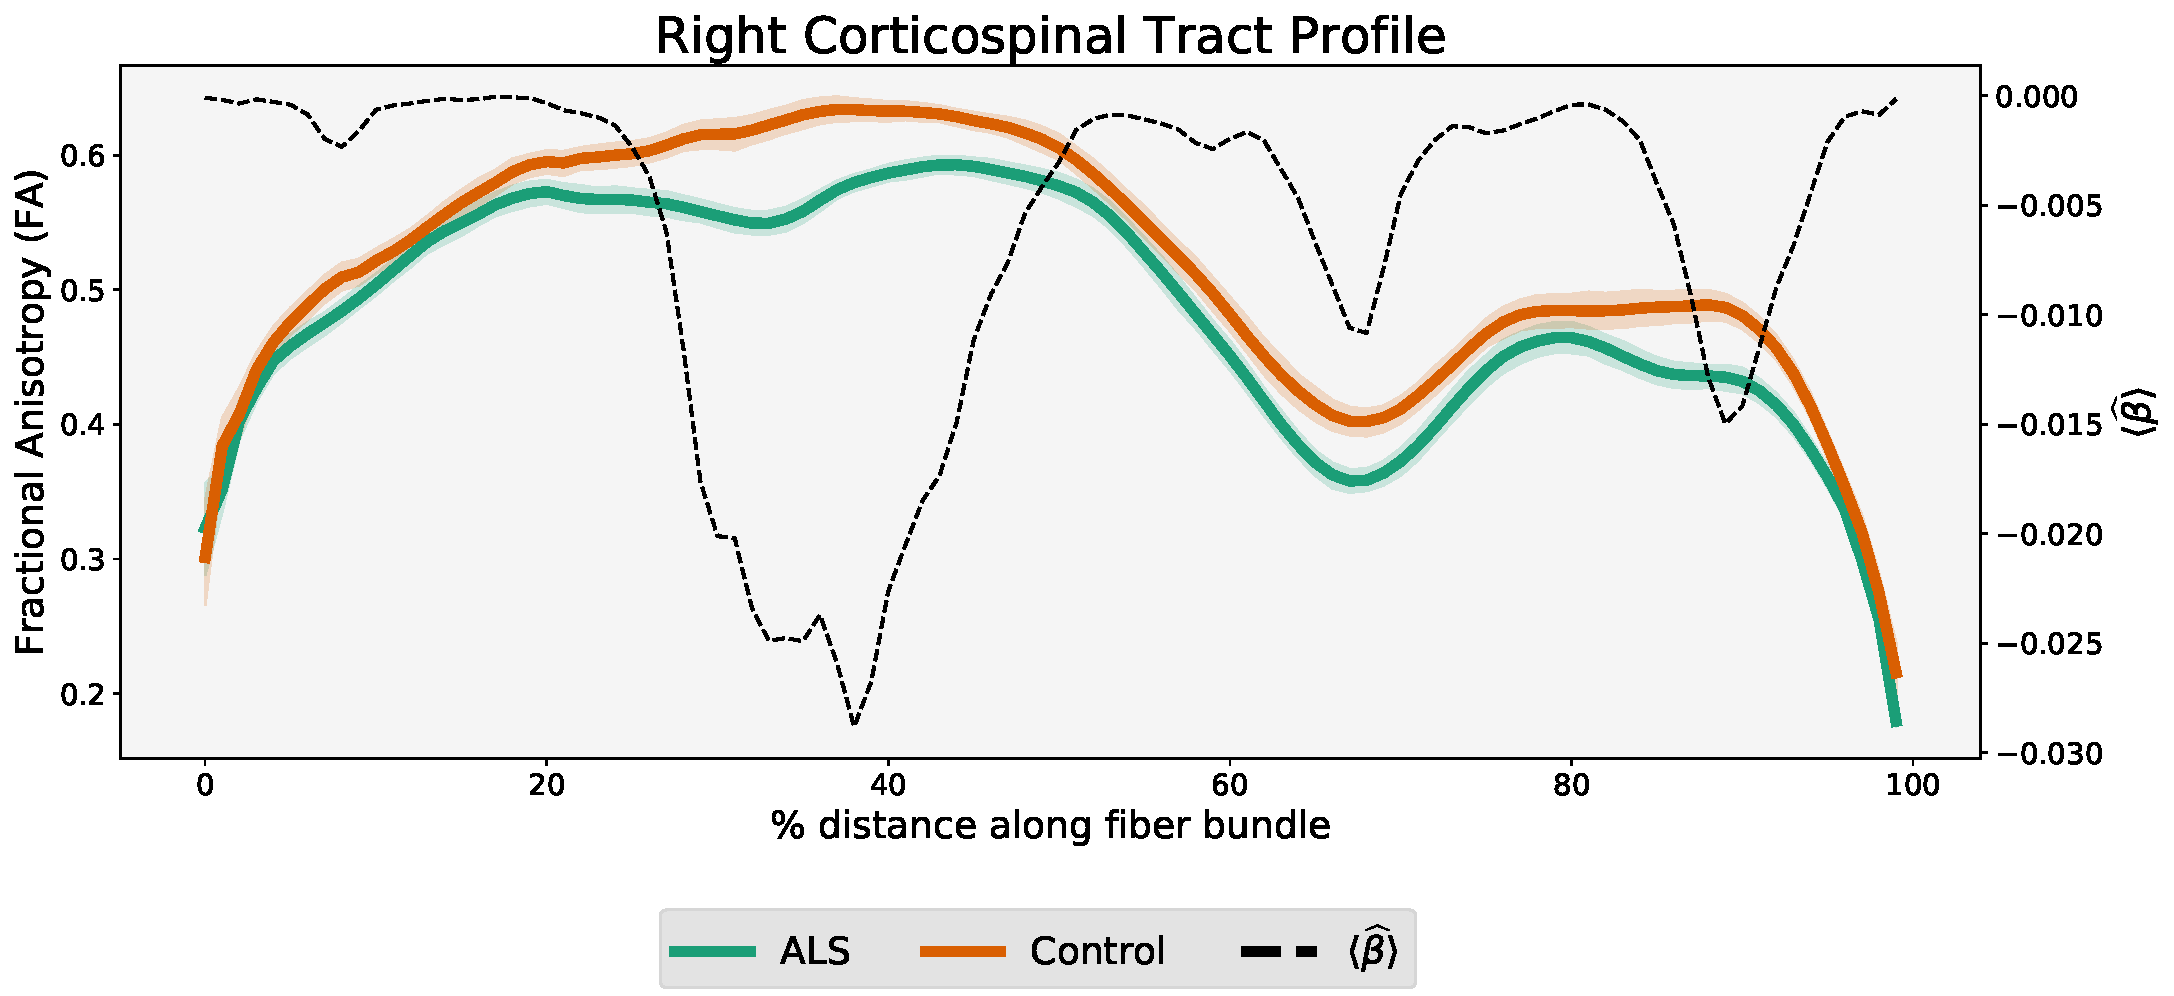
\includegraphics[width=0.95\textwidth]{classification_tract_profiles.pdf}
    \caption{{\bf Model coefficients mirror FA differences}. The places along the
       length of the CST  where $\hat{\beta}$ coefficients for FA
       (dashed line, right axis) have large negative values correspond to the
       locations of substantial differences between the ALS (green) and control
       (orange) FA (shaded area indicates standard error of the mean).}
    \label{fig:class-profiles}
\end{figure}


\begin{figure}[!h]
    \centering
        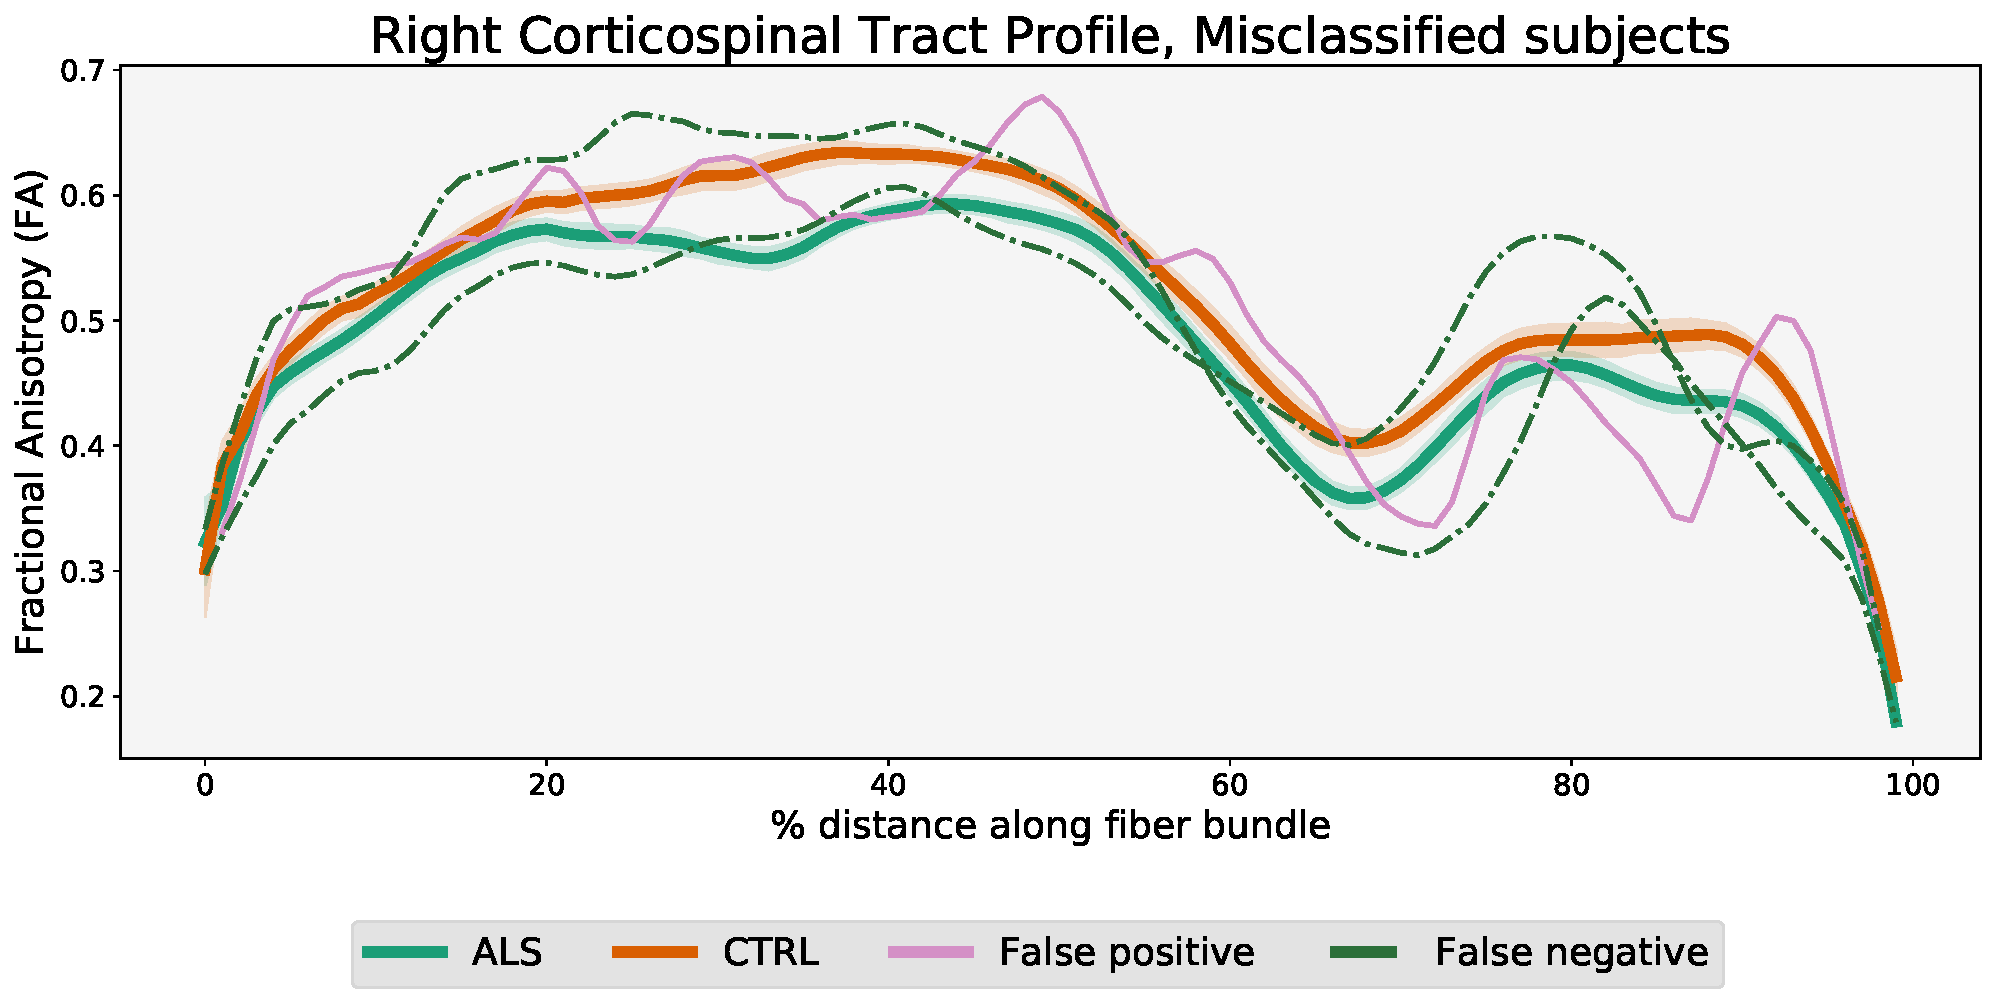
\includegraphics[width=0.95\textwidth]{classification_subjects_profiles.pdf}
    \caption{{\bf Model mis-classifications correspond to features identified by
       the model}. The FA in CST of individuals that are mis-classified by the
       model is compared the group FA (with shaded are indicating standard error
       of the mean). False negative classifications (individuals that have ALS,
       but are classified as patients have) correspond to high FA either in the
       more inferior part of the CST}
    \label{fig:class-errors}
\end{figure}
